%==============================================================================
\chapter{Introduction to Deep Learning}
\label{sec:Deep_learning}
%==============================================================================
Deep learning, as a sub-field of machine learning, is concerned with the study of algorithms that have the ability to learn through experience. The experience is typically gained by presenting the algorithm with data examples from which it learns a set of rules. In the particular case of deep learning, the models considered are Deep Neural Networks (DNNs). \\
In this chapter, Artificial Neural Networks (ANNs) are introduced first before turning to the more advanced DNNs. Two different types of DNNs, namely Feedforward Neural Networks (FNNs) and Recurrent Neural Networks (RNNs) and their training algorithms will be discussed. Furthermore, different types of activation functions, weight initializations, and optimization algorithms are reviewed. Special emphasis is put on the application to \textit{supervised classification tasks} which is the kind of problem at hand in the latter chapters of this thesis. 

\section{Artificial Neural Networks}
\label{sec:ANNs}
\begin{figure}[H]
\centering
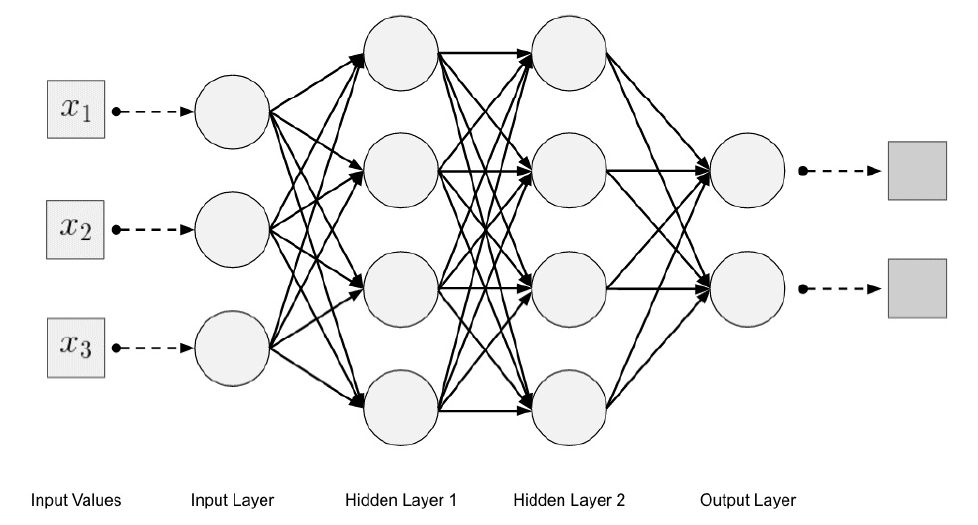
\includegraphics[scale=0.37]{figs/NeuralNetwork.png}
\caption{Schematic structure of a deep neural network with fully connected layers. The input values of the given task $x_i$ are fed into the neurons (depicted as circles) of the input layer and processed in the hidden layers. The weights which connect neurons located at different layers are represented by a solid arrow. In the output layer, all information is combined and predictions (depicted as dark squares) about the classes are made. (Figure taken from \cite{patterson2017deep})}
\label{fig:NeuralNetwork}
\end{figure}
As it is often the case for inventions in science and technology, the idea of ANNs is inspired from nature, more precisely by the human brain. The two key principles involved in the decision-making process of human brains are recognizing patterns and inductive thinking \cite{logan2018thinking}. These, for any machine learning model, highly desirable attributes, are modeled by imitating the structure of the human brain in an ANN. \\
The basic building blocks of the brain, neurons, process and transmit information via electric and chemical signals. The input signals received by a neuron is summarized to a net input $z$. This net input is then compared to an internal threshold. The output of the neuron is 1 if the threshold is passed and 0 otherwise. Since the summarization process of all the input signals to the net input is still part of on going research in the field \cite{bioNeuron}, the net input $z$ for artificial neuron is simply defined to be
\begin{equation}
z=b + \sum_i x_i w_i
\end{equation}
where $w_i$ are weights representing the assigned importance of the different features $x_i$, b is the bias term which is the the artificial equivalent of the threshold in a biological neuron. Additionally, an arbitrary \textit{activation function} $\Phi(z)$ is applied to the net input corresponding to the unknown degrees of freedom in the decision-making process and determining the final output of the artificial neuron. \\
The neurons in an ANN are structured as layers, shown in Figure \ref{fig:NeuralNetwork}. The first layer is called the \textit{input layer}, containing all the input features. In practice, these input features are physical variables such as kinematic quantities of the final state particles. The layers following the input layer are called \textit{hidden layers}. If an ANN has more than one hidden layer it is considered a DNN and thus, by definition a deep learning model. The different layers are connected to their successors via weight vectors $\vec{w}$. Depending on the magnitude of the weights a neuron can focus on a combination of features provided by the neurons in the previous layer. The model complexity and flexibility, therefore, increases with the number of neurons $n$ and layers $\ell$ it contains. In the case of fully connected layers, i.e. every neuron in a given layer is connected to all neurons in the previous layer, the number of free parameters (weights and bias) can be calculated according to
\begin{equation}
\sum_{\ell=1}^{L} n^{\ell-1} n^{\ell} + n{^\ell}
\label{eq:NumPara}
\end{equation}
where $L$ is number of layers in the Neural Network. The last layer is called the \textit{output layer} where all information is compressed and predictions are made. In this thesis, the prediction made is the affiliation of an event to a signal or background process. In terms of machine learning language, such a problem is called a \textit{supervised classification task} where the supervision is given by the correct assignment known from the simulation. To get the classification right, an ANN has to learn which combination of features ultimately results in the best separation between the different classes. This process is often referred to as \textit{training} and is discussed in the next section.

\section{Training of Feed-Forward Neural Networks}
\label{sec:training}
There are several different types of Neural Network, each adjusted and optimized for their specific field of application. However, they all share a similar, gradient-based training procedure that can be best understood considering Feed-Forward Neural Networks\footnote{The name originates from the fact that, in an FNN information is always passed forward. Different types of ANNs also involve a cyclic flow of information within one neuron (see section \ref{sec:RNN})} (FNNs). \\
The first step of any gradient-based method is the \textit{forward pass}. The forward pass involves the evaluation of the net input and the activation function for each neuron successively. The neuron output values $a=\Phi(z)$ are preserved for the necessary gradient calculations later in the training. The forward pass is applied for each event individually such that the predictions made in the output layer results in a prediction distribution $p$. This distribution is used to evaluate the current performance of the neural network based on a \textit{loss function}.

\newpage
\paragraph{Loss function} \mbox{} \\
The loss function $L(\theta)$ is a measure of how close $p$ is to the true distribution $y$, and depends on the weight tensor $\theta$ which includes all trainable parameters\footnote{The bias term can be reinterpreted as the weight $w_0 = -1$ of the weight tensor \cite{NNTheory}}. The training of an FNN is said to have converged if the trainable parameters are adjusted such that the loss function is at its global minimum i.e. for all events the predicted probability is as close as possible to the true class. \\
A  commonly chosen loss function for classification task is the cross-entropy loss \cite{Crossentro} defined for $K=2$ classes and m events as
\begin{equation}
L(\theta) = - \frac{1}{m} \sum^{m}_{i=1} \sum^{K}_{j=1} y^{(i)}_{j} \cdot \ln(p^{(i)}_{j}) = - \frac{1}{m} \sum^{m}_{i=1} [y^{(i)} \ln(p^{(i)}) + (1-y^{(i)})\ln(1-p^{(i)})]
\label{eq:crossent}
\end{equation}
where $p^{(i)}_{j}$ is the predicted probability that the $i^{th}$ event belongs to class $j$ and $y^{(i)}_{j}$ is either 1 if the true class of the event is j or 0 otherwise. It can be derived from the Kullback-Leibler Divergence \cite{Kulldiv} and thus interpreted as the likelihood that $p$ could have been generated by $y$. Selecting the cross-entropy loss avoids small values in the gradient calculations which is key for fast convergence of the training algorithm discussed in the next sub-section.

\paragraph{Backpropagation algorithm} \mbox{} \\
The most widely used training algorithm is called the Backpropagation algorithm \cite{backpro}. In addition to the first forward pass, a second backward pass is performed. In the backward pass, weight updates for each weight in the ANN are calculated based on the neuron outputs obtained in the forward pass. The exact execution of the weight updates depends on the optimization algorithm chosen. Nevertheless, most optimization algorithms are variations of the simple gradient descent method. Gradient descent calculates the partial derivatives of the loss function for each weight, exploiting the chain rule. In the case of the cross-entropy loss for a single event, the derivative with respect to the weight between the $j^{th}$ neuron in layer $\ell$ and the $k^{th}$ neuron in previous layer $\ell-1$ is given by
\begin{equation}
\label{eq:part_deriv}
\frac{\partial L}{\partial w^{\ell}_{jk}} =  \frac{1}{n} \sum_{k=0}^n x^{\ell-1}_{k} (\phi(z^{\ell}_{j})-y_{j}) 
\end{equation} 
where the predicted distribution $p$ in Equation \ref{eq:crossent} was expressed as a function of the $n$ output features $a^{\ell-1}_{k}$ provided by the neurons in the previous layers. Equation \ref{eq:part_deriv} only holds for particular choices of the activation function for instance the sigmoid function $\frac{1}{1+e^{-z}}$. This often-used activation function can be especially problematic since its derivation leads to vanishing gradients. However, since the partial derivative of the cross-entropy is independent of the neuron's output derivative, this problem can be avoided. Hence, gradient descent, in combination with cross-entropy, ensures fast convergence of the weight updates. The weight updates themselves are performed by adjusting the current weight 
$w^{\ell}_{jk}(t-1)$ to the new weight $w^{\ell}_{jk}(t)$ via
\begin{equation}
\label{eq:WeightUpdate}
w^{\ell}_{jk}(t) = w^{\ell}_{jk}(t-1) - \alpha \cdot \frac{\partial L}{\partial w^{\ell}_{jk}}
\end{equation}
where $\alpha$ is a tunable hyperparameter called the \textit{learning rate} which determines the step size of the learning updates. \\
One complete iteration of the Backpropagation algorithm is called an \textit{Epoch}. It comprises of the forward pass, the evaluation of the loss function, and updates of the weights based on a gradient method such as gradient descent. Typically an FNN needs to be trained over several Epochs to obtain a well-separating model.

\section{Recurrent Neural Networks}
\label{sec:RNN}
\begin{figure}[H]
\centering
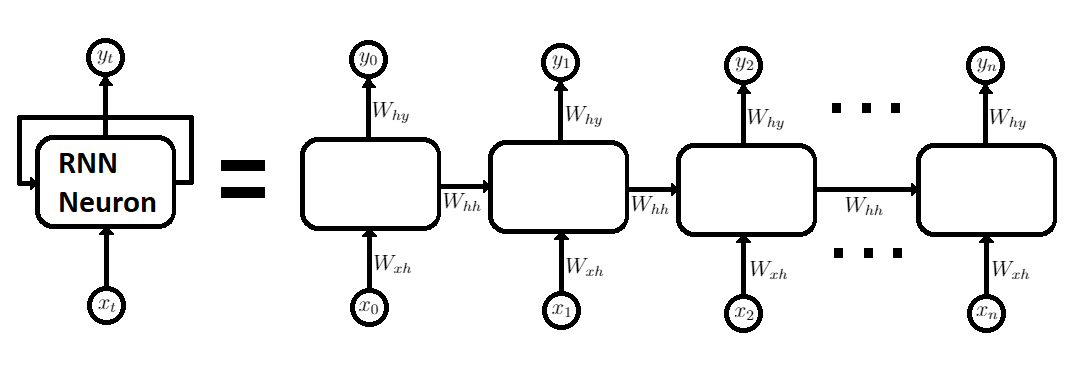
\includegraphics[scale=0.58]{figs/Unrolling.png}
\caption{Schematic description of a Recurrent Neural Network neuron unrolled through time. The information is propagated in a feed-forward manner using the same three weight matrices at each time step.}
\label{fig:unrolling}
\end{figure}
Even though FNNs have outperformed human experts in numerous tasks \cite{NNbH1,NNbH2,NNbH3}, they still lack some fundamental capabilities of the brain. One of which is the ability to remember. To solve this problem Recurrent Neural Networks (RNNs) were introduced. The input features of RNNs are ordered data sequences of varying lengths. RNNs are most prominently capable of understanding and making up meaningful sentences. However, RNNs can also be utilized in physics applications when measurements can be organized as a sequence. For instance, by ordering final state particles of the same type according to their transverse momenta discussed in more detail in Section \ref{sec:feature_selection}. \\
The neurons of an RNN have at least one additional state called the \textit{hidden state}. This state functions as a feedback loop in time connecting the data earlier in the sequences with their successors.
Thus, important information for the context is available at all times. Figure \ref{fig:unrolling} shows the hidden state loop unrolled in time. Each time-step is a copy of the same neuron receiving a different part of the sequence as input $x_i$. Every copy of the neuron is connected with its descendent by the same weight matrix $w_{hh}$. Consequently, the update of the hidden state vector $\vec{h}(t-1)$ to the new hidden state $\vec{h}(t)$ can be expressed as
\begin{equation}
\vec{h}(t) = \Phi(w_{hh} \vec{h}(t-1) + w_{xh} \vec{x})
\end{equation}
where $w_{xh}$ is the weight matrix connecting the input vector $\vec{x}$ with the hidden state and $\Phi$ the activation function. The individual outputs $y_i$ are connected with the current hidden state $h_i$ via the weight matrix $w_{hy}$ and therefore can be calculated as
\begin{equation}
y_i = w_{hy} \cdot h_i
\end{equation}
The training of the weight matrices is performed by the Backpropagation Through Time algorithm (BTT). Similar to the standard Backpropagation algorithm, BTT propagates the gradient backward from the output to the input layer. Additionally, the BTT propagates the gradients also backward in time. \\
While the above-described RNNs can in principle retain information over a long sequence, in practice the calculated gradient quickly vanishes, rendering the training impossible. The solution to this problem comes with the Long Term Short Memory (LSTM) neuron architecture which introduces one more intermediate state called the \textit{cell state}. A LSTM neuron performs four basic iterations at each time step. Firstly the irrelevant parts in the current cell state are forgotten based on the new information and the old hidden state. Then, new information that is relevant for processing the sequence is stored, followed by updating the cell state based on the results obtained. Lastly, the output to the hidden state is computed based on the updated cell state and the new information. \\
The cell state has the advantage that it allows for an uninterrupted flow of the gradients and therefore makes it possible to process long sequential data.

\section{Optimization of Neural Networks}
\label{sec:optimization}
At the base of optimization of Neural Networks is the ``no free lunch theorem''. It states that there is no one single model that works for every problem \cite{patterson2017deep}. The only way to build ANNs with high performance is to try out different optimization algorithms, activation functions, weight initializations, and so forth. Hence, after introducing the performance measure of choice, the most commonly used options will be discussed in this section.

\paragraph{Performance measures} \mbox{} \\

\begin{figure}[H]
\begin{subfigure}{.33\textwidth}
  \centering
  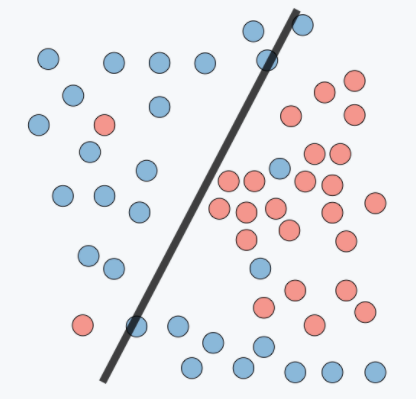
\includegraphics[width=.8\linewidth]{figs/underfitting.png}
  \caption{Underfitting }
  \label{fig:Underfitting}
\end{subfigure}%
\begin{subfigure}{.33\textwidth}
  \centering
  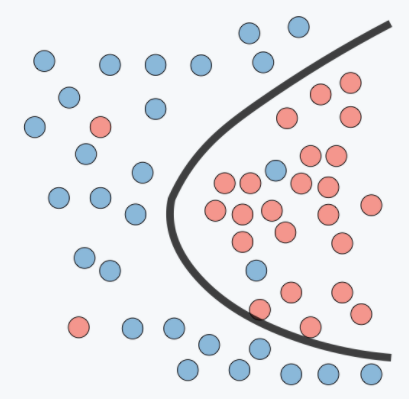
\includegraphics[width=.8\linewidth]{figs/goodfitting.png}
  \caption{Appropriate-fitting}
  \label{fig:Appropriatefitting}
\end{subfigure}
\begin{subfigure}{.33\textwidth}
  \centering
  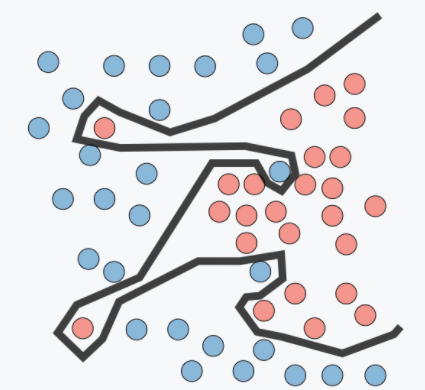
\includegraphics[width=.8\linewidth]{figs/overtraining.png}
  \caption{Overfitting}
  \label{fig:Overfitting}
\end{subfigure}
\caption{Three different models (black) to distinguish the red from the blue circles. \cite{OVPic}}
\label{fig:fitting}
\end{figure}

%Receiver-Operator-Characteristic (ROC) Curve
In this thesis, most of the time binary classification problems are considered where an event either belongs to the signal class or the background class. Therefore, when evaluating the outcome of the classification four cases are possible
\begin{enumerate}[leftmargin=3.5cm]
\setlength{\itemsep}{1pt}
\item[\textbf{True positive (TP):}] The true and the predicted class is signal
\item[\textbf{False negative (FN):}] The true class is signal but the predicted class is background
\item[\textbf{False positive (FP):}] The true class is background but the predicted class is signal
\item[\textbf{True negative (TN):}] The true and the predicted class is background
\end{enumerate}
These quantities can be summarized using the Receiver-Operator-Characteristic (ROC) curve where the signal efficiency ($x = \frac{\text{TP}}{\text{TP}+\text{FN}}$) is plotted against the background rejection ($y =1 - \frac{\text{FP}}{\text{TN}+\text{FP}}$). The separation power of the classifier is then given by $\Gamma$, the Area Under the Curve (AUC) which is the integral under the ROC curve. A model that is capable of distinguishing all signal events from all background events has an AUC of 1. However, in practice, models with such high AUC are very likely to overfit the dataset used during training. Overfitting also called overtraining, schematically depicted in Figure \ref{fig:Overfitting}, occurs when the model is too complex and not only detects subtle patterns of the data but also of the noise. One way of reducing overfitting is to decrease the number of parameters used in the neural network. This is achieved by simplifying its architecture i.e. the number of layers and neurons. On the other hand, a random classifier, which on average gets 50\% of the event classes correctly, achieves an AUC of 0.5. A model that is too simple to parametrize the underlying structure of the data underfits the problem, as shown in Figure \ref{fig:Underfitting}. In the case of Neural Networks there are various ways of avoiding underfitting such as selecting a more complex architecture or adjusting the \textit{learning rate} of the optimization algorithm.

\newpage

\paragraph{Optimization algorithms} \mbox{} \\
Gradient Descent discussed in Section \ref{sec:training} is just one choice of the optimization algorithm. In practice, Gradient Descent is rarely used due to its high computational cost. A very popular variation is the mini batch Stochastic Gradient Descent (SGD) \cite{MainNN}. SGD calculates the weight updates based on a small randomly selected subset of the dataset, called the \textit{batch}.The number of events in the batch the  \text{batch size} and is a hyperparameter of a Neural Network. The full statistics of the dataset is used by calculating the weight updates $m$ times until all events in the dataset were used. The number of batches $m$ is given by batch size divided by the number of events in the total dataset. One evaluation of the weight upgrades on the batch will be refereed to as an \textit{iteration}. The usage of SGD can decrease the computational cost significantly. Furthermore, due to the random nature of the batch selection, the training algorithm can escape local minima in the weight space more easily than the Gradient Descent. \\
Two problems that can similarly slow down the training process are saddle points and plateaus where the gradient and therefore the weight updates can become very small or very large. An optimization algorithm designed to increase the performance of Neural Networks in such situations is the RMSprop \cite{Opti}. This algorithm introduces a constant step size where the direction of the weight update depends on the sign of the gradient. The constant step size is only changed if the previous and the current gradients have the same sign. In this case the step size $v_t$ for the next weight update $w_t$ is given by the previous step size $v_{t-1}$ multiplied with a constant factor $\beta$
\begin{equation}
v_t = \beta v_{t-1}+(1-\beta)(\frac{\partial L}{\partial w})^2
\end{equation}
\begin{equation}
w_t = w_{t-1}-\frac{\alpha}{\sqrt{v_t}} \frac{\partial L}{\partial w}
\end{equation}
where the name giving root mean squared term (RMS) is needed to incorporate mini-batches for the gradient calculation. \\
An optimization algorithm that has been shown to work well for a broad range of applications is the Adaptive Moment Estimation (ADAM) algorithm \cite{Opti}. Like RMSprop it uses $v_t$ term while introducing an additional term $m_t$ called the momentum term. This term ensures a faster convergence by increasing the learning rate for those weights that had a large contribution in the previous step
\begin{equation}
m_t = \beta_2 m_{t-1} + (1-\beta_2) \frac{\partial L}{\partial w}
\end{equation}
where $\beta_2$ is a constant scaling factor. The weight update for ADAM is than given as
\begin{equation}
w_t = w_{t-1}-\frac{\alpha}{\sqrt{\bar{v}_t}} \bar{m_t}
\end{equation}
where $\bar{v_t} = \frac{v_t}{1 - \beta}$ and $\bar{m_t} = \frac{m_t}{1 - \beta_2}$ are bias corrections needed to counteract the initialization to 0. \\
As always in machine learning the best choice of the hyperparameters such as learn rate, scaling factors, and batch size can only be found by testing.

\newpage

\paragraph{Activation functions and Weight initialization}  \mbox{} \\

\begin{figure}[H]
\begin{subfigure}{.5\textwidth}
  \centering
  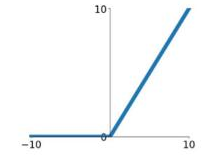
\includegraphics[width=.8\linewidth]{figs/Relu.png}
  \caption{ReLU}
  \label{fig:Relu}
\end{subfigure}%
\begin{subfigure}{.5\textwidth}
  \centering
  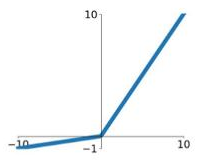
\includegraphics[width=.8\linewidth]{figs/leakyRelu.png}
  \caption{Leaky ReLU}
  \label{fig:LeakyRelu}
\end{subfigure}
\begin{subfigure}{.5\textwidth}
  \centering
  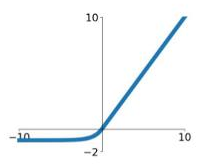
\includegraphics[width=.8\linewidth]{figs/Elu.png}
  \caption{ELU}
  \label{fig:ELU}
\end{subfigure}
\begin{subfigure}{.5\textwidth}
  \centering
  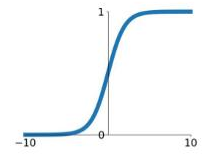
\includegraphics[width=.8\linewidth]{figs/sigmoid.png}
  \caption{Sigmoid}
  \label{fig:Sigmoid}
\end{subfigure}
\caption{Four commonly used activation functions \cite{Acti}}
\label{fig:activfunc}
\end{figure}

Another component of a neural network that can have a big influence on its performance is the activation function. The \textit{rectified linear} (ReLU) activation function, shown in Figure \ref{fig:Relu}, inherits the net input for positive values and evaluates to 0 otherwise. Consequently, the weight updates are easy to compute or cancel completely. This can be an advantage when it comes to computation cost, and a disadvantage if the obtained performance is poor. The \textit{leaky} ReLU activation function (Figure \ref{fig:LeakyRelu}) is similar to ReLU, except for negative values where it returns the net input scaled by a constant $\alpha$. Thus, all weights are updated in each iteration which for some cases improves the performance. The Exponential Linear Unit (ELU), is shown in Figure \ref{fig:ELU}, is very similar to leaky ReLU but has a smooth transition between negative and negative net input values. Its defined as
\begin{equation}
\label{eq:selu}
\text{selu}(z) = \lambda \begin{cases}
z &\text{if}\,\, z < 0 \\
\alpha e^{-z}-\alpha &\text{if}\,\, z \geq 0
\end{cases}
\end{equation}
$\lambda$ is fixed two 1 and $\alpha$ is a tunable parameters. A special version of ELU is the Scaled Exponential Linear Unit (SELU) which was designed to improve the performance of FNNs. The SELU activation function fixes $\alpha$ to 1.6732 and $\lambda$ to 1.0507. The sigmoid activation function (Figure \ref{fig:Sigmoid}) can take values between 0 and 1 and hence is the preferred choice for the output layer where probabilities for the different classes are obtained. Moreover, it's the activation function that is closest to the initial idea of the biological neuron whose output is either 0 or 1. One drawback of the sigmoid activation function is related with its exponential definition (see Section \ref{sec:training}). Calculating exponential functions is much more computationally challenging then computing linear functions like ReLU. \\
Closely related to the selection of the activation function is the choice of the weight initialization. For instance some activation function like SELU require normal distributed weight initialization. The simplest choice would be to initialize all weights and biases to a constant value. However, this leads to the same partial derivative for all weights and thus only one feature could be learned. Therefore, it's not surprising that weight initialization can have a considerable influence on the performance of a neural network. The most popular methods are LeCun, Glorot, and He initialization. These methods draw random values for the initial weights from uniform or normal distribution. They only differ, in upper and lower bounds or standard deviation and mean. The biases, on the other hand, are typically initialized separately either to 0, a small constant value, or 1 in the case of LSTMs.

\paragraph{Regularization} \mbox{} \\
\label{sec:regularization}
The methods and functions described previously all try to increase the performance measure. Another way of improving a Neural Network is to decreasing its overtraining. This process is referred to as \textit{regularization}. The straightforward way of decreasing the overtraining is to reduce the number of parameters. However, removing neurons or entire layers might lead to a completely different training behavior. Two other regularization strategies that avoid changes in the architecture are the Ridge Regression \cite{rigde} and Lasso Regression \cite{lasso} also called $\ell$1 and $\ell$2 regularization. Both introduce additional terms to the loss function. In the case of  Lasso Regression, this term is given by the $\ell$1 norm $\alpha_1 \sum_{i=1}^{n} |w_i|$ where $\alpha_1$ is a new hyperparameter and $w_i$ is the $i^{th}$ weight. A useful property of this regularization is that it tends to eliminate the weights for the least important features. The term of the Ridge Regression is defined as the $\ell$2 norm $\alpha_2 \sum_{i=1}^{n} |w_i|^2$. For large $\alpha_2$, all weights are close to zero, thus reducing the degrees of freedom. \\
Another approach to avoid overtraining is the method of \textit{Dropout} \cite{dropout}. In this method, at each training step, every neuron has a probability $t$ to be temporarily ignored, meaning that it will not forward any output signals to it is successor neurons. Hence, Dropout prevents the neural network to rely too much on specific neurons.
